% -*- root: main.tex -*-

\chapter{Mapowanie obiektowe}

Jedną z~największych zalet relacyjnych baz danych w~kontekście programowania obiektowego jest dostępność bibliotek, które umożliwiają proste mapowanie obiektowo-relacyjne\footnote{W~dalszej części pracy używany będzie skrót ORM od angielskiego pojęcia object-relational mapping.}. Wykorzystanie ORM znacząco upraszcza proces tworzenia oprogramowania wykorzystującego bazy danych:

\begin{itemize}
	\item Umożliwia definiowanie modelu danych poprzez tworzenie klas reprezentujących obiekty wykorzystywane w~aplikacji.
	\item Zarządzanie połączeniami, sesjami i~transakcjami bazodanowymi jest znacząco uproszczone lub dokonywane automatycznie.
	\item Zwiększa bezpieczeństwo aplikacji. Mechanizmy ORM dostarczają narzędzi do ochrony przez atakami typu SQL Injection\footnote{SQL Injection (ang. wstrzykiwanie SQL) - typ ataku polegający na wykorzystywaniu specjalnie spreparowanych wartości, które dołączone do szablonu zapytania SQL powodują szkodliwe działania niezgodne z~intencją programisty.}.~\cite{orm_sql_injection_protection}
	\item Umożliwia modyfikacje środowiska bazodanowego bez zmieniania kodu aplikacji. Mechanizmy ORM wspierają wiele silników bazodanowych, które mogą różnić się od siebie implementowanymi standardami języka SQL. 
\end{itemize}

O~popularności mechanizmów ORM świadczy fakt powstawania oficjalnych standardów mapowania obiektowo-relacyjnego włączanych do specyfikacji języków programowania. Przykładem takiego standardu jest JPA\footnote{Java Persistence API.} dla języka Java.

\section{Mapowanie obiektowo-relacyjne dla Cassandry}

Wraz z~pojawieniem się języka CQL pojawiła się szansa wykorzystania istniejących implementacji mechanizmów ORM do przechowywania danych z~użyciem silnika Cassandry. Motywacją do stworzenia takiego rozwiązania jest zwiększenie wydajności istniejących aplikacji bez modyfikacji ich kodu. Minimalna rekonfiguracja aplikacji i~podłączenie jej pod klaster bazodanowy skutkowałyby zwiększeniem wydajności działania aplikacji. Ponadto wykorzystanie istniejących interfejsów mogłoby umożliwić obsługę różnych typów baz danych należących do ruchu NoSQL. 

Przykładem projektu, który wykorzystuje mechanizm ORM do obsługi NoSQLowych baz danych jest Kundera.\cite{kundera_home} Kundera zapewnia implementację mapowania obiektowego zgodną ze standardem JPA 2.0 między innymi dla Cassandry, HBase, MongoDB oraz Neo4j. Dodatkowo biblioteka wspiera obsługę wielu mechanizmów równocześnie.

\subsection{Kundera - wydajność}

Wyniki pomiarów na stronie domowej projektu Kundera świadczą o~tym, że biblioteka nie wprowadza znacznych narzutów wydajnościowych względem bezpośredniego wykorzystania interfejsu bazy danych. W~przypadku wykorzystania mechanizmów mapowania obiektowo-relacyjnego w~odniesieniu do Cassandry należy zbadać jaki narzut związany jest z~modelowaniem dziedziny danych przy ich pomocy. Do pomiarów wykorzystano dwa modele: przedstawiony na diagramie~\ref{fig:er_wishlist} oraz~\ref{tab:denormalized_wishlist}. Pierwszy model został opisany w~standardzie JPA i~uruchomiony dla Cassandry oraz relacyjnej bazy danych. Drugi model bezpośrednio wykorzystuje CQL. Dla obu wariantów zostały przeprowadzone dwa testy: wstawianie oraz odczytywanie elementów z~bazy danych. 

W~trakcie testów został zmierzony całkowity czas wykonania danej operacji. Przyjęte zostały następujące założenia:

\begin{itemize}
	\item Liczba użytkowników i~przedmiotów są parametryzowane i~skalowane liniowo.
	\item Liczba przedmiotów, które użytkownik może mieć na swojej liście życzeń zawiera się w~przedziale $[0;10]$.
	\item Odczytywana jest parametryzowalna liczba użytkowników.
\end{itemize}

\begin{figure}
	\centering
	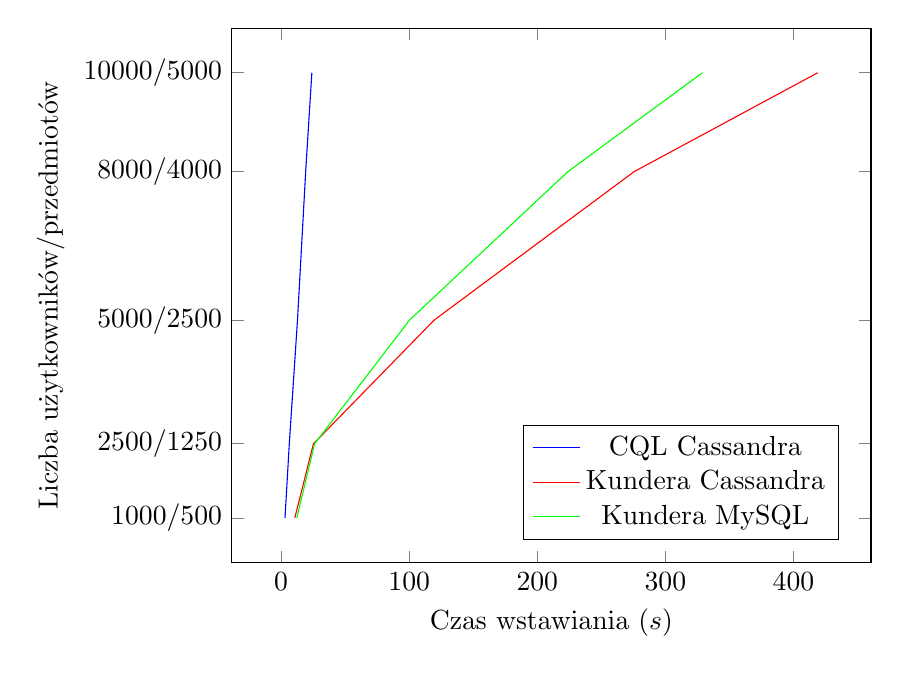
\begin{tikzpicture}
		\begin{axis}[
				width=.8\textwidth,
				xlabel=Czas wstawiania ($s$),
				ylabel=Liczba użytkowników/przedmiotów,
				scaled ticks=false, 
				tick label style={/pgf/number format/fixed},
				ytick={1000, 2500, 5000, 8000, 10000},
				yticklabels={1000/500, 2500/1250, 5000/2500, 8000/4000, 10000/5000},
				legend style={at={(0.95,0.15)},anchor=east}
			]
			\addplot[color=blue] coordinates {
				(23.978, 10000)
				(19.155, 8000)
				(12.762, 5000)
				(6.366, 2500)
				(3.005, 1000)
			};
			\addlegendentry{CQL Cassandra}

			\addplot[color=red] coordinates {
				(418.915, 10000)
				(275.532, 8000)
				(119.453, 5000)
				(25.213, 2500)
				(10.657, 1000)
			};
			\addlegendentry{Kundera Cassandra}

			\addplot[color=green] coordinates {
				(328.915, 10000)
				(223.823, 8000)
				(100.23, 5000)
				(26.119, 2500)
				(12.232, 1000)
			};
			\addlegendentry{Kundera MySQL}
		\end{axis}
	\end{tikzpicture}

	\caption{Porównanie czasu wstawiania wielu rekordów.}
\end{figure}

\begin{figure}
	\centering
	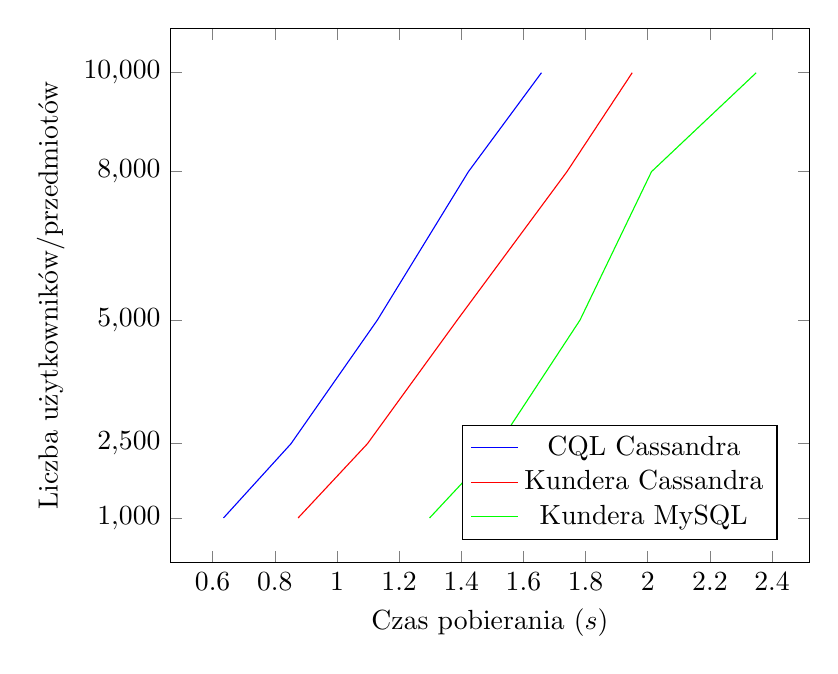
\begin{tikzpicture}
		\begin{axis}[
				width=.8\textwidth,
				xlabel=Czas pobierania ($s$),
				ylabel=Liczba użytkowników/przedmiotów,
				scaled ticks=false, 
				tick label style={/pgf/number format/fixed},
				ytick={1000, 2500, 5000, 8000, 10000},
				legend style={at={(0.95,0.15)},anchor=east}
			]
			\addplot[color=blue] coordinates {
				(1.658, 10000)
				(1.423, 8000)
				(1.130, 5000)
				(0.852, 2500)
				(0.635, 1000)
			};
			\addlegendentry{CQL Cassandra}

			\addplot[color=red] coordinates {
				(1.95, 10000)
				(1.74, 8000)
				(1.387, 5000)
				(1.098, 2500)
				(0.875, 1000)
			};
			\addlegendentry{Kundera Cassandra}

			\addplot[color=green] coordinates {
				(2.349, 10000)
				(2.012, 8000)
				(1.782, 5000)
				(1.521, 2500)
				(1.298, 1000)
			};
			\addlegendentry{Kundera MySQL}
		\end{axis}
	\end{tikzpicture}

	\caption{Porównanie czasu pobierania wielu rekordów.}
\end{figure}